\section{Introduction}
This paper has been written for the course Managing Big Data at the University of Twente. The goal of this paper is to explain the preparation, execution and results of the project we performed for this course. The project required us to perform operations on a large data set, and use the results for the purpose of answering a research question. Several data sets were made available to us on the CTIT cluster at the University of Twente. 

We decided to use the Twitter data that is provided by Twiqs.nl, which contains a large part of the Dutch tweets from the period of December 2010 until November 2015. Twiqs aims to collect all tweets that are sent in The Netherlands or have a Dutch language. The tweets are filtered by language, only the tweets that are determined to be Dutch by an algorithm of Twiqs are included in the data set. Because of Twitter API limits not all tweets are collected, but estimations by Twiqs indicate that around 80\% is collected.

We wanted to research the Twitter data in the gaming area, in order to see if there is any relation between the number of tweets about a certain game (especially around the release date) and the number of copies that a game sells. Therefore the research question is as follows:
\textit{Does the number of tweets about a game relate to the number of copies sold in Europe?}

For the number of copies that a game sells, we will use the top 20 sold games from the video game sales chart on the website called VGChartz \footnote{http://www.vgchartz.com/} and filter this list to find the games that are released since 2011. The reason why we are filtering this list from the year 2011 onward is because the Twitter data also spans the period from 2011 until now. The filtered and ordered list on sales in Europe can be found in Table \ref{resultNumbers}. This list will be used during this research.

To get some first impressions about the data, we have used the web interface of Twiqs to search through the Twitter data. We have searched for ‘witcher’ (which is supposed to catch the game ‘The Witcher 3’) in the time period of January 1st, 2015 until December 31st, 2015 to see if we could find the release date. Twiqs searched in 288480444 tweets with this term and time period, and found 12032 tweets. The results show a clear peak around the end of May, which corresponds to the release date of May 19th, 2015. We also searched for ‘battlefield’, ‘fifa 15’ and ‘minecraft’ to get some more examples of game data. Out of our examples we can conclude that we can find enough tweets to find something meaningful.
\begin{figure}[!ht]
	\centering
		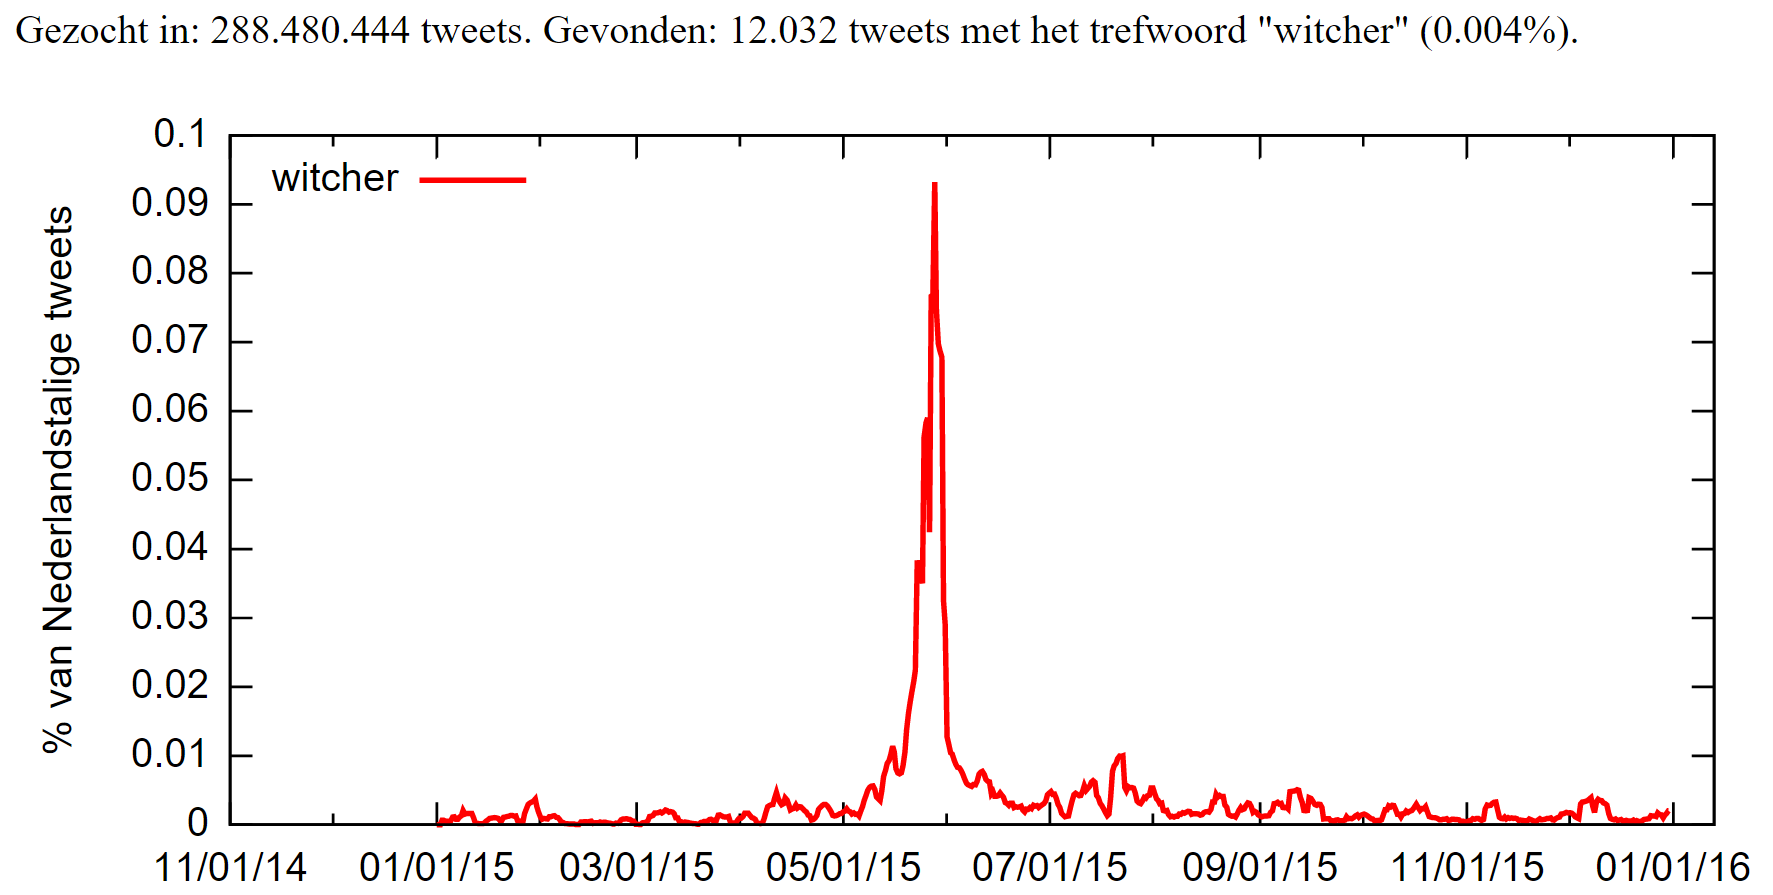
\includegraphics[width=0.476\textwidth]{twiqswitcher}
	\caption{Search on Twiqs.nl for ‘witcher’ in the period of January 2015 until December 2015.}
\end{figure}
\subsection{Need}
The results of the research will confirm or deny that there is a relation between the amount of copies that were sold and the number of tweets about the game in the release year. This relation would be useful for game publishers, game developers, game review sites and customers. For example, if there exists such a relation, then the amount of tweets that are sent at the time of release could potentially be an indicator for the estimated amount of copies that will be sold for the game. This data could be useful for publishers and developers, as it will show them the amount of excitement and interest that is being displayed for their game upon release.
\subsection{Task}
With use of MapReduce we will search in all available tweets and count the number of tweets that are about a certain game. These counts will include time data so that grouping can be used on a certain scale to get a good graph for the number of tweets related to time. It will probably make sense to group data per day. 
\subsection{Preprocessing}
The following operations will be performed on the tweet text and search terms before using them:
convert to lowercase;
remove all punctuation;
remove all whitespace characters.
These operations will ensure that we need just a few variations of the search terms, and that the search results are a lot more consistent. Using the lowercase versions makes sense because we do not want to search for each casing, and changing to lowercase does not introduce any (or at least an unnoticeable number) false positives. Removing punctuation also helps, as official review sites will often use official names like \textit{Call of Duty: Advanced Warfare}, but customers will likely not use punctuation in this way, so the special characters from these need to be removed so that they match the search terms. Removing special characters also ensures that we take Twitter hashtags into consideration while running the job. Removing whitespace is possible because having the words of a game name directly after each other does not make any existing word, so it is not likely to appear in a tweet that is not referring to the game.
\subsection{Further steps}
A next step would be to determine the list of games from the Twitter data itself, instead of searching with a predefined list. Game names could be scanned for by checking for the words before/after the word ‘game’. Then this game list could be used as input for the initial program to calculate the score for each game. Challenges for automatically determining the list of games would be finding the names, and keeping the list clean. This is hard because normally game names are not mentioned with a certain term in front or after it, so it is not trivial to find these.
\subsection{Expected results}
The result of this research will consist of comparisons between the amount of tweets that have been created about a game and its sales records. The results of the amount of tweets and the sales records will be visualized as a graph and will usually show a peak in the amount of tweets sent around the time of a game’s release date. The answer to our research question depends on whether there is a correlation between the amount of tweets that have been sent and the amount of copies that were sold.


